% link to instruction: https://tc.computer.org/tcde/tcde-bulletin-author-instructions/
\documentclass[11pt]{article} 
% \usepackage[utf8]{inputenc}

\usepackage{deauthor,times}
\usepackage{graphicx} % 
\usepackage{hyperref}
\usepackage{wrapfig}
% \usepackage{comment}
% \graphicspath{{asudeh/}}
\usepackage{amsfonts,amsmath}



% Use \begin{document} immediately before the title and authors are given.
\begin{document}

% \title{Responsible Scoring and Ranking by Human-designed and Machine-learned Algorithms}
\title{Towards Responsible Data-driven Decision Making in Score-Based Systems
\footnote{This work was supported in part by NSF Grants No. 1741022 and 1926250.}
}
\author{Abolfazl Asudeh\footnotemark[2], H. V. Jagadish\footnotemark[3], Julia Stoyanovich\footnotemark[4] \\
\footnotemark[2]  University of Illinois at Chicago, \footnotemark[3] University of Michigan, \footnotemark[4] New York University\\
\footnotemark[2] {asudeh@uic.edu}, \footnotemark[3] {jag@umich.edu}, \footnotemark[4] {stoyanovich@nyu.edu}
}
% \date{}

\maketitle


\begin{abstract}
Human decision makers often receive assistance from data-driven algorithmic systems that provide a {\em score} for evaluating the quality of items such as products, services, or individuals. These scores can be obtained by combining different features either through a process learned by ML models, or using a weight vector designed by human experts, with their past experience and notions of what constitutes item quality. The scores can be used for different evaluation purposes such as ranking or classification.

% may be derived in different ways.  For example, they may be learned from training data, or computed as a linear combination of attribute values, using a weight vector specified by a human expert.   We refer to the entities that determine how an item is to be scored as {\em evaluators}.  An evaluator may be a human expert, with her past experience and notions of what constitutes item quality, or it may be a machine that learns how to score items based on training data.  

%can be obtained by combining different features through a complex black-box process learned by ML models,  or by linearly combining some decision attributes, using a weight vector designed by human experts or machine-learned using some training data.  

%In this paper we view decision making in score-based systems through the lens of responsibility.
%
%While using these systems 
%can help make society safer, more just, and more prosperous, irresponsible implementation of these technologies may not only fail to help, but even harm us on an unprecedented scale.
%

In this paper, we view the design of these scores through the lens of responsibility.  %We consider human experts (for human-designed evaluators) and training data (for machine-learned evaluators) as key factors to achieve responsible data-driven decision making,
%Viewing the experts and training data as the key factors for human-designed and machine-learned scores, 
We present technical methods (i) to assist human experts in designing fair and stable score-based rankings and (ii) to assess and (if needed) enhance the coverage of a training dataset for machine learning tasks such as classification.
% present technical methods for assisting (human) experts in designing scoring methods that lead to fair and stable rankings.  We also present algorithms that help machine evaluators assess  the coverage of a training dataset for a task such as classification, and mitigate the lack of coverage when necessary.
 \end{abstract}
\section{Introduction}  
\label{s:intro}
The past decade has observed a surge in the design and deployment of 
decentralized systems. A key reason for this surge is the growing desire in 
the society to have self-governing democratic financial systems that are not 
under the control of a privileged set of entities. A central control often 
translates to a forced trust model with limited provision to support 
transparency and accountability. The adoption of Blockchain, for example, 
is a by-product of the ability to break away from the forced-central control 
in a trust-worthy fashion~\cite{blockchain-book}. The emerging blockchain 
platforms facilitate a reliable execution of any digital contracts 
(i.e., transactions) in a decentralized manner despite the existence of malicious 
actors. At the core of any blockchain platform is a Byzantine 
fault-tolerant (\BFT{}) consensus protocol and a tamper-proof replicated 
ledger~\cite{bedrock,blockchain-book,scalable-ledger}. The \BFT{} 
protocol helps to achieve {\em consensus} on the order of incoming client 
requests among all the replicas, while the ledger logs this agreement. 

Traditional \BFT{} protocols expect a {\em permissioned} system where the 
identities of all the replicas (i.e., participants) are known prior to any 
consensus as they rely on having a verifiable voting right in a democratic 
setting. These protocols rely on a {\em communication-oriented} consensus 
model, where all the participants exchange endorsements across multiple 
rounds before they can reach a decision~\cite{sharper,pbftj,ahl,poe,rcc,geobft,flexitrust,ringbft,mirbft,basil,hotstuff}.
In these protocols, a system of $\n{}$ replicas can reach a common decision 
if at most $\f{}$ of them are malicious, such that $\n{} \ge 3\f{}+1$. 
The $\n{}$ parties are said to reach a decision when at least a majority 
of honest parties agrees to that decision. This decision is logged by 
requiring all the agreeing parties to {\em sign} the decision. Hence, the 
reached decision is considered {\em tamper-proof} because it has support 
of a majority of honest participants.

Despite being around for more than two decades, traditional \BFT{} protocols 
did not see any major practical applications until the introduction of 
blockchain technology. We attribute {\em two} key factors for this lack of 
adoption. (i) To ensure that the malicious participants do not spawn multiple 
identities, these \BFT{} protocols need an authority (i.e., {\em a forced 
trust gateway}) to verify and register every participant to verify every 
vote~\cite{sybil-attack}; some participants may find this intrusive if they 
do not want to reveal their personal information. (ii) To overwrite the ledger, 
malicious participants just require access to the private keys of honest 
participants. In a sense, the proof of the validity of the ledger is not 
self-contained, and it operates on the assumption that the private-keys 
are kept safe externally indefinitely.

To resolve these challenges, initial blockchain platforms such as 
Bitcoin~\cite{bitcoin} and Ethereum~\cite{ether} offer a {\em permissionless} 
model of consensus. These systems employ the {\em Proof-of-Work} (\PoW{}) 
protocol~\cite{bitcoin,ether}, which follows a {\em computation-oriented} 
consensus model and requires all the participants to compete with each other 
and try to solve a complex puzzle. Whichever participant solves the puzzle 
first gets to add a new entry ({\em block}) to the ledger. As a result, 
\PoW{} protocol eliminates the three challenges seen by traditional \BFT{} 
protocols. (i) Malicious participants can spawn multiple identities, but what 
actually matters is the available compute power. (ii) Each block includes 
the hash of the previous block; overwriting the ledger requires recomputing 
all the blocks making it computationally infeasible. (iii) Since reaching the 
consensus is based on presenting the proof of work that is embedded on the 
ledger (i.e., self-contained), there is no longer any need for external 
safe-keeping of private keys to sign endorsements.

These properties offered by \PoW{} protocol help blockchain platforms to 
design a {\em decentralized economy}, where any person can participate in the 
consensus process, and the economy has a self-generating currency to monetize 
its participants. Monetizing the participants is necessary as the \PoW{} 
protocol expects the participants to spend their resources to solve a complex 
puzzle. Clients of the Bitcoin platform, create transactions that exchange 
Bitcoins and send them to the participants (miners) in the \PoW{} protocol. 
These miners check if the transaction is valid; the client has sufficient 
Bitcoins to transfer. If the transaction is valid, they run \PoW{} protocol to include 
this transaction in the ledger. The winning miner of \PoW{} gets a portion of 
the client's Bitcoin as {\em fees}, while the mining process (\PoW{}) mints  
new tokens to fund the economy. This new token is transferred to the winning 
miner's account and is recorded as a transaction in the block.

The key challenge with platforms like Bitcoin is their {\em practicality}. 
These platforms have abysmally low throughput in the order of $10$ transactions 
per second in part due to inadequate choice of small block sizes. Furthermore, as 
more miners join the network, the complexity of the puzzle has to be increased. 
For example, the complexity of the current Bitcoin puzzle is so high that the 
miners work in large groups to have any positive probability of creating the 
next winning block~\cite{blockchain-book}. Moreover, as miners are competing 
with each other, it leads to massive wastage of computational resources (energy) 
as only the winning miner's efforts are recorded and rewarded. This results in an unsustainable ecosystem~\cite{badcoin,badbadcoin}.

We observe these challenges in the designs of existing \BFT{} protocols and 
blockchain platforms and envision a \DualChain{} system that learns from these 
models and eliminates their key challenges. Essentially, we aim to establish a 
new research agenda; a new field of hybrid consensus protocols that depart from 
competitive consensus to a collaborative consensus that is both resilient and 
sustainable. Our \DualChain{} architecture takes a step in this direction by 
running two consensuses on each client transaction while ensuring there is no 
increase in the latency observed by the client. Each client request is first 
ordered through a state-of-the-art \BFT{} consensus protocol ({\em commitment}), 
subsequently, this ordered request is engraved into the ledger through the 
\PoW-style consensus ({\em settlement}). Specifically, \DualChain{} causes no 
increase in commitment latency while improving the settlement latency observed 
by existing protocols. Ordering the client transaction through a \BFT{} consensus 
protocol first allows our \DualChain{} system to guarantee the following benefits: 
(i) clients receive low-latency responses, and (ii) \PoW{} participants no longer 
need to compete, resulting in a high-throughput sustainable chain. As a result, 
instead of employing the \PoW{} for consensus, we design a novel protocol that 
allows miners to collaborate. We refer to this paradigm as 
{\em Power-of-Collaboration} (\PoC{}). 

Our \PoC{} protocol splits the complex puzzle into disjoint slices and requires 
each miner to work on a distinct slice. This slice distribution significantly 
reduces the resource wastage and provides each honest miner with a reward 
for each new transaction added to the ledger. As each ledger entry is added 
collaboratively, any malicious entity that wishes to overwrite the ledger 
needs to match the computational power of all the existing miners making it 
practically impossible. These features of our \DualChain{} system make it 
lucrative; its design is the bedrock for a secure and efficient decentralized 
economy.

\section{Responsible Ranking}\label{sec:ranking}
Ranking of individuals is commonplace today, and is used, for example, for college admissions and employment. 
% Properly, topics such as ranking, top-$k$ query processing, and building indexes to efficiently answer such queries, have recently been increasingly relevant to database research.
Score-based evaluators, designed by human experts, are commonly used for ranking, especially when there are multiple criteria to consider.
The scores are usually computed by linearly combining (with non-negative weights) the relevant attributes of each individual from some dataset $\mathcal{D}$. Then, we sort the individuals in decreasing order of score and finally return either the full ranked list or its highest-scoring sub-set, the top-$k$. 

Formally, we consider a dataset $\mathcal{D}$ to consist of $n$ items, each with $d$ scalar scoring attributes. In addition to the scoring attributes, the dataset may contain non-scoring attributes that are used for filtering, but they are not our concern here.  Thus we represent an item $t \in \mathcal{D}$ as a $d$-length vector of scoring attributes, $\langle x_1, x_2, \ldots, x_d \rangle$.  Without loss of generality, we assume that the scoring attributes have been appropriately transformed: normalized to non-negative values between 0 and 1, standardized to have equivalent variance, and adjusted so that larger values are preferred.
A {\em scoring function} $f_{\vec{w}}: \mathbb{R}^d\rightarrow\mathbb{R}$, with weight vector $\vec{w} ~ = ~\langle w_1, w_2,\ldots,w_d \rangle$, assigns the score $f_{\vec{w}}(t) = \Sigma_{j=1}^d w_j t[j]$ to any item $t\in\mathcal{D}$.

Linear scoring functions are straightforward to compute and easy to understand~\cite{asudeh2016query}.
That is the reason they are popular for ranking, and for evaluation in general.
However, it turns out that the rankings may highly depend on the design of these functions.
To further explain this, let us consider the following toy example.

\begin{example}\label{example1}
\em
Consider a real estate agency with two offices in Chicago, IL and Detroit, MI.
The owner assigns agents based on need (randomly) to the offices.
By the end of the year, she wants to give a promotion to the ``best'' three agents.
The criteria for choosing the agents are $x_1:$ {\tt \small sales} and $x_2:$ {\tt \small customer satisfaction}.
Figure~\ref{fig:toyexample:data} shows the values in $\mathcal{D}$, after normalization.
Considering the two criteria to be (roughly) equally important, the owner chooses the weights $\vec{w}=\langle 1, 1 \rangle$ for scoring. That is, the score of every agent is computed as $f=x_1+x_2$.
The 5th column in Figure~\ref{fig:toyexample:data} shows the scores, based on this function.
According to function $f$, the top-3 agents are $t_6$, $t_4$, and $t_2$, with scores 1.4, 1.38, and 1.37, respectively. 
Note that, according to $f$, all top-3 agents are located in Chicago and no agent from Detroit is selected.
\end{example}

\begin{figure*}[!tb]
\begin{minipage}[t]{0.39\textwidth}
\centering
\small
\vspace{-38mm}
    \begin{tabular}{|l|c|c|@{}c@{}||@{}c@{}|@{}c@{}|}
	\hline
	\multicolumn{4}{|c||}{$\mathcal{D}$} & $f$&$f'$ \\ \hline
	id   & $x_1$ & $x_2$ & location&$ \; \langle 1, 1 \rangle \;$&$\langle 1.11, .9 \rangle$ \\ \hline \hline
	$t_1$& 0.63 & 0.71&Detroit&1.34&1.338 \\ \hline
	$t_2$& 0.72 & 0.65&Chicago&1.37&1.384 \\ \hline
	$t_3$& 0.58 & 0.78&Detroit&1.36&1.387 \\ \hline
    $t_4$& 0.7 & 0.68&Chicago&1.38&1.389 \\ \hline
	$t_5$& 0.53 & 0.82&Detroit&1.35&1.321 \\ \hline
	$t_6$& 0.61 & 0.79&Chicago&1.4&1.388 \\ \hline
	\end{tabular}
    \vspace{-1mm}\caption{Example~\ref{example1}-Data}
    \label{fig:toyexample:data}
\end{minipage}
\hfill
\begin{minipage}[t]{0.32\textwidth}
\centering
    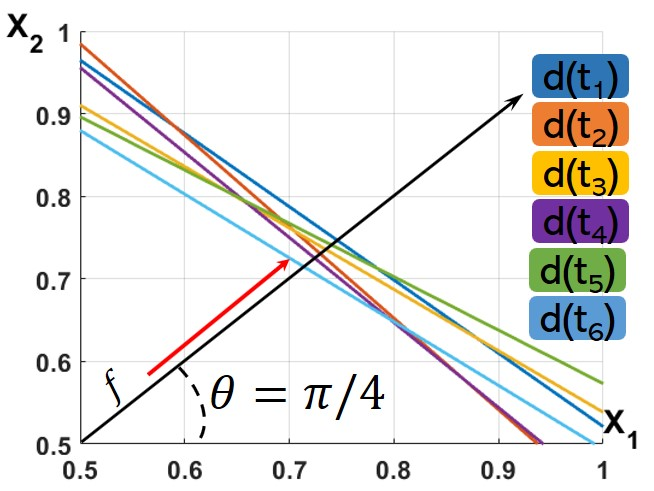
\includegraphics[width=\textwidth]{figs/dualspace.jpg}
    \vspace{-10mm}\caption{Example~\ref{example1}-Dual space}
    \label{fig:toyexample:dual}
\end{minipage}
\hfill
\begin{minipage}[t]{0.25\textwidth}
\centering
    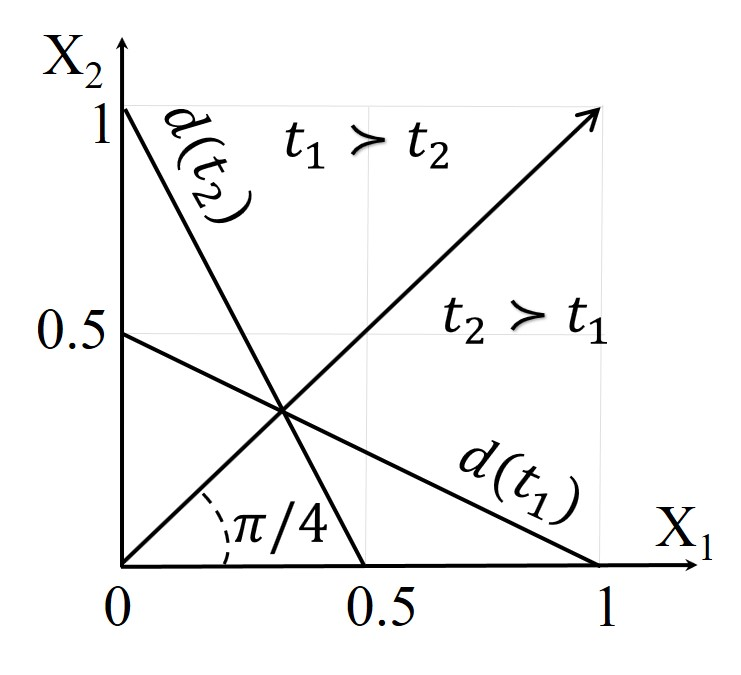
\includegraphics[width=\textwidth]{figs/orderingexchange.jpg}
    \vspace{-10mm}\caption{Ordering exchange between $t_1$:[1,2] and $t_2$:[2,1]}
    \label{fig:orderingexchange}
\end{minipage}
\vspace{-8mm}
\end{figure*}

The specific weights chosen have a huge impact on the score and hence rank for an item.
In Example~\ref{example1}, the owner chose the weight vector $\vec{w}=\langle 1, 1 \rangle$, {\em in an ad-hoc manner}, without paying attention to the consequences.
However, small changes in the weights could dramatically change the ranking. 
For example, the function $f'$ with the weight vector $\vec{w'}=\langle 1.1, .9 \rangle$ may be equally good for the owner and she may not even have a preference between $\vec{w}$ and $\vec{w}'$. Probably her choice of weights is only because $\vec{w}$ is more intuitive to human beings.
The last column in Figure~\ref{fig:toyexample:data} shows the scores based on $f'$, which produce the ranking $f': \langle t_4, t_6, t_3, t_2, t_1, t_5\rangle$. Comparing it with the ranking generated by $f:  \langle t_6, t_4, t_2, t_3, t_5, t_1\rangle$, one may notice that the rank of each and every individual has changed. More importantly, while according to $f$ all promotions are given to the agents of the Chicago office, $f'$ gives two promotions to Chicago and one to Detroit.

Many sports use ranking schemes. An example is the FIFA World Ranking of national soccer teams based on  recent performance.
FIFA uses these rankings as ``a reliable measure for comparing national A-teams''~\cite{fifa}. 
Despite the trust placed by FIFA in these rankings, many critics have questioned their validity.
University rankings is another example that is both prominent and often contested~\cite{Gladwell11Order}: various entities, such as U.S. News and World Report, Times Higher Education, and QS, produce such rankings.  Similarly, many funding agencies compute a score for a research proposal as a weighted sum of scores of its attributes. These rankings are, once again, impactful, yet heavily criticized.
Similarly, in criminal justice, COMPAS~\cite{propublica} was originally intended to provide services and positive interventions, under resource constraints.  That is, a score computed by COMPAS would then be used to rank individuals to prioritize access to services.
Many other impactful examples can be mentioned, such as a company that evaluates its employees to promote some and let go some others, and a college admissions officer who decides to admit a small portion of the applicants.

Surprisingly, similar to Example~\ref{example1}, despite the enormous impact of score-based rankers, attribute weights are usually assigned in an ad-hoc manner, based only on intuitive reasoning and common-sense of the human designers.
For instance, in the case of FIFA rankings, the scoring formula combines  the past four years  of performance of each team as $x_1+0.5x_2+0.3x_3+0.2x_4$, where $x_i$ is the team's performance in the past $i^{th}$ year. Of course, the designers tried to come up with a set of weights that make sense. For them $0.98x_1+0.51x_2+0.29x_3+0.192x_4$ would probably be equally acceptable, since the weight values are virtually identical: they choose the former formula simply because round numbers are more intuitive.
This issue, in the context of university ranking, is further elaborated by Malcolm Gladwell in~\cite{Gladwell11Order}.

Assuming that the designers of rankings are willing to accept scoring functions similar to their initial functions, Mithra provides a toolbox and algorithms to help human experts practice responsible ranking. In the following, we start by providing some necessary background from computational geometry in \S~\ref{sec:bgnd}, followed by an explanation of fairness and stability in our framework in \S~\ref{sec:defs}.

\subsection{Fairness and Stability Models}\label{sec:defs} % 1 page
Decisions based on rankings may impact the lives of individuals and even influence societal policies. For this reason, it is essential to  make the development and deployment of rankings transparent and otherwise principled.
Also, since rankings highly depend on what weights are chosen in the scoring function, it is necessary to make sure that generated rankings are fair and robust.

\subsubsection{Fairness}
There is not a single universal definition of fairness.  
Impossibility theorems~\cite{friedler2016possibility} have established that we cannot simultaneously achieve all types of fairness.
Indeed, the appropriate definitions of fairness greatly depend on the context and on the perspective of the user. Sometimes, it may even be prescribed by law. 
As such, we consider a general definition of fairness in our work. Our focus is on societal (v.s. statistical) bias~\cite{narayanan2018translation} and group fairness~\cite{hardt2016equality2} (v.s. individual fairness~\cite{dwork2012fairness2}).

We consider some attributes, used for decision making (e.g. sales and customer satisfaction in Example~\ref{example1}), to be {\em non-sensitive}. Some other attributes, such as race and gender (and location in Example~\ref{example1}), we consider to be {\em sensitive}.
We adopt the Boolean fairness model, in which a fairness oracle $\mathcal{O}$ takes as input an ordered list of items from $\mathcal{D}$, and determines whether the list
satisfies a set of {\em fairness constraints}, defined over the sensitive attributes: $\mathcal{O}: \mathcal{r}_f(\mathcal{D}) \rightarrow \{\top, \bot\}$. A scoring function $f$ that gives rise to a fair ordering over  $\mathcal{D}$ is said to be {\em satisfactory}.
For instance, in Example~\ref{example1}, assume that the owner knows that, because of some hidden factors, sales and customer satisfaction patterns are different in Chicago and Detroit. Hence, she considers the selection of the top-3 agents to be fair, if it assigns at least one of the promotions to each one of the offices. Note that according to this criterion, the ranking provided by $f=x_1+x_2$ is not fair as it assigns all three promotions to the agents in Chicago.
On the other hand the ranking generated by function $f'=1.1x_1+.9x_2$ assigns two of the promotions to Chicago and one to Detroit, and hence is considered to be fair. 


\subsubsection{Stability}
We want a ranking to be {\em stable} with respect to changes in the weights used for scoring.  Given a particular ranked list of items, one question a consumer will ask is: how robust is the ranking? If small changes in weights can change the ranked order, then there cannot be much confidence in the correctness of the ranking. We call a ranking of items {\em stable} if it is generated by a large portion of scoring functions in the neighborhood of the initial scoring function specified by the expert. 

Every scoring function in a universe $\mathcal{U}^*$ of scoring functions induces a single ranking of the items. But each ranking is generated by many functions.
For a dataset $\mathcal{D}$, let $\mathfrak{R}_\mathcal{D}$ be the set of rankings over the items in $\mathcal{D}$ that are generated by at least one scoring function $f\in\mathcal{U}^*$. 
Consider the set of scoring functions that generate a ranking $\mathfrak{r}\in\mathfrak{R}_\mathcal{D}$.
Because this set of functions is continuous, we can think of it as a region in the space of all possible functions in $\mathcal{U}^*$.
We use the region associated with a ranking to define the ranking's stability. The intuition is that a ranking is stable if it can be induced by a large set of functions.
If the region of a ranking is large, then small changes in the weight vector are not likely to cross the boundary of a region and therefore the ranked order will not change. 
For every region $R$, let its volume, $vol(R)$, be the measure of its bulk.
Given a ranking $\mathfrak{r}\in\mathfrak{R}_\mathcal{D}$, the stability of $\mathfrak{r}$ is the proportion of scoring functions in $\mathcal{U}^*$ that generate $\mathfrak{r}$.
That is, stability is the ratio of the volume of the ranking region of $\mathfrak{r}$ to the volume of $\mathcal{U}^*$. Formally:
\begin{align}
S_\mathcal{D}(\mathfrak{r}) = \frac{\mbox{vol}(R_\mathcal{D}(\mathfrak{r}))}{\mbox{vol}(\mathcal{U}^*)}
\end{align}
We emphasize that stability is a property of a ranking (not of a scoring function).


\subsection{Geometric Interpretation}\label{sec:bgnd} %0.5 pages
In the popular geometric model for studying data, each attribute is modeled as a dimension and items are interpreted as points in a multi-dimensional space.
We transform this {\em Primal space} into a {\em dual space}~\cite{edelsbrunner}.
%, where every item corresponds to a hyperplane.

We use the dual space in $\mathbb{R}^d$, where an item $t$ is presented by a hyperplane $\mathsf{d}(t)$ given by the following equation of $d$ variables $x_1 \dots x_d$:
\vspace{-5mm}
\begin{align}\label{eq:dual}
\mathsf{d}(t):~ t[1]\times x_1 + \dots + t[d]\times x_d = 1
\end{align}

Continuing with Example~\ref{example1}, Figure~\ref{fig:toyexample:dual} shows the items in the dual space. In $\mathbb{R}^2$, every item $t$ is a 2-dimensional hyperplane (i.e. simply a line) given by $\mathsf{d}(t): t[1] x_1 + t[2] x_2=1$.
In the dual space, a scoring function $f_{\vec{w}}$ is represented as a ray starting from the origin and passing through the point $[w_1, w_2,...,w_d]$.
For example, the function $f$ with the weight vector $\vec{w}=\langle 1,1 \rangle$ in Example~\ref{example1} is drawn in Figure~\ref{fig:toyexample:dual} as the origin-starting ray that passes through the point $[1,1]$. Note that every scoring function (origin-starting ray) can be identified by $(d-1)$ angles $\langle \theta_1, \theta_2, \cdots, \theta_{d-1} \rangle$, each in the range $[0,\pi/2]$. Thus, given a function $f_{\vec{w}}$, its angle vector can be computed using the polar coordinates of $w$.
For example, the function $f$ in Figure~\ref{fig:toyexample:dual} is identified by the angle $\theta=\pi/4$.
There is a one-to-one mapping between these rays and the points on the surface of the origin-centered unit $d$-sphere (the unit hypersphere in $\mathbb{R}^d$), or to the surface of any origin-centered $d$-sphere.
Thus, (the first quadrant of) the unit $d$-sphere represents the universe of functions $\mathcal{U}$.

Consider the intersection of a dual hyperplane $\mathsf{d}(t)$ with the ray of a function $f$.
This intersection is in the form of $a\times\vec{w}$, because every point on the ray of $f$ is a linear scaling of $\vec{w}$.
Since this point is also on the hyperplane $\mathsf{d}(t)$,
$t[1]\times a\times w_1 + \dots + t[d]\times a\times w_d = 1$. Hence, $\sum t[j] w_j = 1/a$. This means that the dual hyperplane of any item with the score $f(t)=1/a$ intersects the ray of $f$ at point $a\times\vec{w}$.
Following this, the ordering of the items based on a function $f$ is determined by the ordering of the intersection of the hyperplanes with the vector of $f$. The closer an intersection is to the origin, the higher its rank.
For example, in Figure~\ref{fig:toyexample:dual}, the intersection of the line $t_6$ with the ray of $f=x_1 + x_2$ is closest to the origin, and $t_6$ has the highest rank for $f$.

Consider the dual presentation of two items $t_1:[1,2]$ and $t_2:[2,1]$, shown in Figure~\ref{fig:orderingexchange}, and a function that passes through this intersection.
We name this function the {\em ordering exchange} between $t_1$ and $t_2$.
That is because this function partitions the space in two regions, where every function in the top-left region ranks $t_1$ higher than $t_2$ while every function in bottom-right ranks $t_2$ higher.
In general, the ordering exchange between a pair of items $t_i$ and $t_j$ is identified by (the set of function on) the following origin-passing hyperplane:
\begin{align}\label{eq:mdIntersect}
\sum\limits_{k=1}^{d} (t_i[k] - t_j[k])w_k = 0
\end{align}



\subsection{Designing Fair Ranking Schemes}\label{sec:fairness2} % 1 page
We interpret fairness to mean that (a) disparate impact, which may arise as a result of historical discrimination, needs to be mitigated; and yet (b) disparate treatment cannot be exercised to mitigate disparate impact when the decision system is deployed. 
Disparate impact arises when a decision making system provides outputs that benefit (or hurt) a group of people sharing a value of a sensitive attribute more frequently than other groups of people.
{\em Disparate treatment}, on the other hand, arises when a decision system provides different outputs for groups of people with the same (or similar) values of non-sensitive attributes but with different values of sensitive attributes. To avoid disparate treatment, it is desirable (and in many cases mandated by law) to not use information about an individual's membership in a protected group as part of decision-making.
Following these, our goal is to build a system that helps human expert to design fair ranking schemes, in the sense that those {\em both} mitigate disparate impact (by ensuring that appropriate proportionality constraints are satisfied) {\em and} do not exercise disparate treatment (by not explicitly using information about an individual's membership in a protected group) during deployment.  That is, a {\em single} evaluator will be used for all items in the dataset, irrespective of their membership in a protected group.

Our goal~\cite{asudeh2019designing} is to build a system to assist a human designer of a scoring function in tuning attribute weights to achieve fairness.
Formally, our {\em closest satisfactory function} problem is:
Given a dataset $\mathcal{D}$ with $n$ items over $d$ scalar scoring attributes, a fairness oracle $\mathcal{O}: \mathcal{r}_f(\mathcal{D}) \rightarrow \{\top, \bot\}$, and a linear scoring function $f$ with the weight vector $\vec{w} = \langle w_1,w_2,\cdots ,w_d\rangle$, find the function $f'$ with the weight vector $\vec{w'}$ such that $\mathcal{O}(\mathcal{r}_{f'}(\mathcal{D}))=\top$  and the angular distance between $\vec{w}$ and $\vec{w'}$ is minimized.

Since the tuning process does not occur too often, it may be acceptable for it to take some time. However, we know that humans are able to produce superior results when they get quick feedback in a design or analysis loop.  Ideally, a  designer of a ranking scheme would want the system to support her work through interactive response times.  Our goal is to meet this need, to the extent possible, by providing a query answering system. From the system's viewpoint, the challenge is to propose similar weight vectors that satisfy the fairness constraints, in interactive time.  To accomplish this, our solution operates with an offline phase and then an online phase.  In the offline phase, we process the dataset, and develop data structures that will be useful in the online phase. 
In the online phase, the user specifies a {\em query} in the form of a scoring function $f$.
If the ranking based on $f$ does not meet the predefined fairness constraints, we suggest to the user an alternative scoring function that is both satisfactory and similar to $f$. The user may accept the suggested function, or she may decide to manually adjust the query and invoke our system once again.

The notion of ordering exchanges, explained in \S~\ref{sec:bgnd} is a key in the preprocessing phase.
Consider the set of ordering exchange hyperplanes between all pairs of items in $\mathcal{D}$.
Similar to Figure~\ref{fig:orderingexchange}, each hyperplane $h_{i,j}$ (the ordering exchange between $t_i$ and $t_j$) partitions the function space $\mathcal{U}$ in two regions where in one region $t_i$ outranks $t_j$ while in the other $t_j$ is ranked higher.
The collection of these hyperplanes provide an arrangement~\cite{redlining} in the form of a dissection of the space into origin-starting connected $d$-cones with convex surfaces, we call {\em ranking regions}. All functions in a ranking region generate the same ranking while every ranking is generated by the functions of (at most) one ranking region.
Hence, in the offline time it is enough to identify the satisfactory ranking regions whose rankings satisfy fairness constraints.

For 2D, we design a raw-sweeping algorithm. At a high level, using a min-heap for maintaining the ordering exchanges, the algorithm sweeps a ray from the $x$ to $y$-axis.
It first orders the items based on the $x$-axis and gradually updates the ordering as it visits an ordering exchange along the way. As the algorithm moves from one ranking region to the other, it checks if the new ranking is fair, and if so, marks the region as satisfactory.
Each satisfactory region in 2D is identified by two angles as its beginning and end.
We construct a the sorted list of (the borders of) satisfactory regions in the offline phase.
Given a query function $f$ in online phase, we apply a binary search on the sorted list. If $f$ falls in a satisfactory region, the algorithm returns $f$, otherwise it returns the closest satisfactory border to $f$.

Discovering the satisfactory regions in MD is challenging when there are more than two attributes.
That is because the complexity of the arrangement of ordering exchanges is exponential in the number of attributes, $d$.
Even given the satisfactory regions, answering user queries in interactive time is not possible. The reason is that we need to solve a non-linear programming problem for each satisfactory region, before answering each query.
To address this issue, we propose an approximation algorithm for obtaining answers quickly, yet accurately.
Our approach relies on first partitioning the function space, based on a user-controlled parameter $N$, into $N$ equi-volume cells, where each cell is a hypercube of $(d-1)$-dimensions.
During preprocessing, we assign a satisfactory function $f_c'$ to every cell $c$ such that, for every function $f$, 
the angle between $f$ and $f_c'$ is within a bounded threshold (based on the value of $N$) from $f$ and its optimal answer.
To do so, we first identify the cells that intersect with a satisfactory region, and assign the corresponding satisfactory function to each such cell. Then, we assign the cells that are outside of the satisfactory regions to the nearest discovered satisfactory function.
In the online phase, given an unsatisfactory function $f$, we need to find the cell to which $f$ belongs, and to return its satisfactory function. 
This can be done in $O(\log N)$ by performing binary searches on the partitioned space.



\subsection{Obtaining Stable Rankings}\label{sec:stability} % 0.75 page
Magnitude of the ranking regions that produces an observed ranking identify its stability.
Stability is a natural concern for consumers of a ranked list.  If a ranking is stable, then the same ranking would be obtained for many choices of weights.  But if this region is small, then we know that only a few weight choices can produce the observed ranking.  This may suggest that the ranking was engineered or ``cherry-picked'' by the producer to obtain a specific outcome. 
Human experts who produce scoring functions for generating the rankings desire to produce stable results.  We argued in~\cite{yang2018nutritional} that stability in a ranked output is an important aspect of algorithmic transparency, because it allows the producer to justify their ranking methodology, and to gain the trust of consumers.
Of course, stability cannot be the only criterion in the choice of a scoring function: the result may be weights that seem ``unreasonable'' to the ranking producer.  To support the producer, we allow them to specify a range of reasonable weights, or an {\em acceptable region} in the space of functions, and help the producer find stable rankings within this region. 

We develop a framework~\cite{asudeh2018obtaining} that can be used to assess the stability of a provided ranking and to obtain a stable ranking within the the acceptable region of scoring functions.
We address the case where the user cares about the rank order of the entire set of items, and also the case where the user cares only about the top-$k$ items.
We focus on efficiently evaluating an operator we call {\sc \small get-next}, which can be used to discover the stable  rankings, ordered by their stability.
Formally, for a dataset $\mathcal{D}$, a region of interest $\mathcal{U}^*$, and the top-$(h-1)$ stable rankings in $\mathcal{U}^*$, discovered by the previous {\sc \small get-next} calls,  our goal is to find the $h$-th stable ranking $\mathfrak{r}\in\mathfrak{R}$.
Note that the {\sc \small get-next} operator enables discovering the top-$\ell$ stable rankings, for any arbitrary $\ell$. That simply can be done by calling the operator $\ell$ times.
Our technical contribution for 2D is similar to the one for fair rankings. The 2D algorithm first discovers the ranking regions in $\mathcal{U}^*$ by sweeping a ray in it. The discovered rankings, along with their stabilities, are moved to a heap data structure. Then, every call of {\sc \small get-next} returns the next stable ranking from heap.

For MD, we design a threshold-based algorithm that uses an arrangement~\cite{asudeh2019designing} tree data structure, AKA cell tree~\cite{tang2017determining}, to partially construct the arrangement of ordering exchange hyperplanes.
Specifically, given that our objective is to find stable rankings and that the user will likely be satisfied after observing {\em a few} rankings,  rather than discovering all possible rankings, we target the discovery of only the next stable ranking and delay the arrangement construction for other rankings. 
Arrangement construction is an iterative process that starts by partitioning the space into two half-spaces by adding the first hyperplane. The construction then iteratively adds the other hyperplanes; to add a new hyperplane, it first identifies the set of regions in the arrangement of previous hyperplanes with which the new hyperplane intersects, and then splits each such region into two new regions. The {\sc \small get-next} operator, however, only breaks down the largest region at every iteration, delaying the construction of the arrangement in all other regions. Please refer to \cite{asudeh2018obtaining} for more details about the algorithm.

While being efficient in practice for medium-size settings, the algorithms based on arrangement construction are not scalable, as their worst-case complexities are cursed by the complexity of the arrangement.
Next, we discuss function sampling as a powerful technique for aggregate estimation using Monte-carlo methods~\cite{montecarlo}, as well as an effective technique for search-space exploration.



\subsection{Function Sampling for Scalability}\label{sec:sampling} % 1 page

Uniform sampling from the scoring function space enables designing randomized algorithms for evaluating and designing score-based evaluators.
In the following, we first discuss sampling from the complete function space and then propose an efficient unbiased sampling from a region of interest $\mathcal{U}^*$.

As explained in \S~\ref{sec:bgnd}, there is a 1-1 mapping between the universe of scoring functions and the points on the surface of (the first quadrant of) the unit $d$-sphere. That is, every point one the surface of the $d$-sphere correspond to a scoring function and vice versa.
Hence, the problem of choosing functions uniformly at random from $\mathcal{U}$ is equivalent to choosing random points from the surface of a $d$-sphere.
As also suggested in~\cite{rrr}, we adopt a method for uniform sampling of the points on the surface of the unit $d$-sphere~\cite{muller1959note, marsaglia1972choosing}.
Rather than sampling the angles, this method samples the weights using the {\em Normal distribution}, and normalizes them. 
This works because the normal distribution function has a constant probability on the surfaces of $d$-spheres with common centers~\cite{marsaglia1972choosing}.
Therefore, in order to generate a random function in $\mathcal{U}$, we set each weight as $w_i = |\mathcal{N}(0,1)|$, where $\mathcal{N}(0,1)$ draws a sample from the standard normal distribution.

In order to compute an aggregate (or conduct exploration) by perturbing in a region of interest $\mathcal{U}^*$ in the neighborhood of some function $f$, we need to only sample from the set of functions with the maximum angle around the ray of $f$.
% More than sampling from the complete function space, our techniques require drawing unbiased samples from a region of interest $\mathcal{U}^*$.
An acceptance-rejection method~\cite{lucidl1989random} can be used for this purpose. That is, to draw a sample, uniformly at random, from $\mathcal{U}$ and accept it, if it belongs to $\mathcal{U}^*$.
The efficiency of this method, however, depends on the volume of $\mathcal{U}^*$, as if it is small, the algorithm will reject most of the generated samples.
Alternatively, we propose a sampler that works based on the following observation:
modeling $\mathcal{U}^*$ as the surface unit $d$-spherical cap, each Riemannian piece of the surface forms a $(d-1)$-sphere.
Following this observation, our sampler first selects a  Riemannian piece, randomly, proportional to its volume. Then it uses the Normal distribution to draw a sample from the surface of the Riemannian piece. 
Please refer to \cite{asudeh2018obtaining} for more details about the design of this sampler.
We would like to emphasize that the proposed sampler has a {\em linear complexity} to the number of attributes $d$. It therefore provides a powerful tool for studying the score-based evaluators in higher dimensions.

We use function sampling for different purposes, including (i) evaluating the stability of a given ranking, (ii) designing a randomized algorithm for finding the stable rankings, and (iii) on-the-fly query processing for discovering fair functions.
For (i) and (ii), in \cite{asudeh2018obtaining}, we design  Monte-carlo methods~\cite{montecarlo} that consume a set of $N$ function samples for finding the rankings in $\mathcal{U}^*$ and computing their stabilities.
For (iii), function sampling provides a heuristics for on-the-fly fair ranking scheme query processing in large-scale settings~\cite{asudeh2019designing}.

We used function sampling in MithraRanking~\cite{guan2019mithraranking}, our web application\footnote{http://mithra.eecs.umich.edu/demo/ranking/}, designed for responsible ranking design.
After uploading a dataset, or choosing among available datasets, the application allows the user to specify the fairness constraints she wants to satisfy.
For instance, in Figure~\ref{fig:MR1}, the user has added a constraint that the top-30\% of the ranking should contain at most 30\% with age more than 56 years old. Note that the interface gives the user the ability to add multiple fairness constraints.
She then, as in Figure~\ref{fig:MR2}, specifies the weight vector of the initial scoring function and a region of interest around it, by specifying a cosine similarity.
The system then ranks the data based on the specified function and checks if the ranking satisfies the fairness criteria. It also draws unbiased function samples from the region of interest to estimate the stability of the generated ranking. The system also uses the samples for finding the most stable rankings in the region of interest, the most similar fair function to the initial function, and a function (not necessarily the most similar) that generates a fair and stable ranking (Figure~\ref{fig:MR3}).
The user can then accept any of those suggestions and change the ranking accordingly.

\begin{figure*}[!tb]
\begin{minipage}[t]{0.32\textwidth}
\centering
    \vspace{-35mm}
    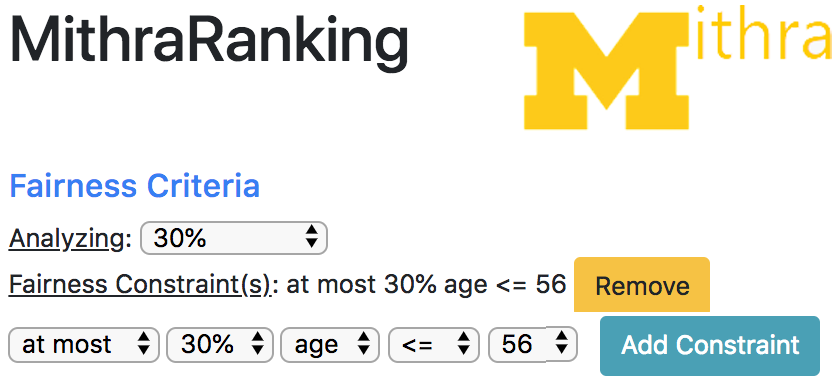
\includegraphics[width=\textwidth]{figs/m2.png}
    \vspace{2mm}\caption{Specifying fairness constraints}
    \label{fig:MR1}
\end{minipage}
\hfill
\begin{minipage}[t]{0.32\textwidth}
\centering
    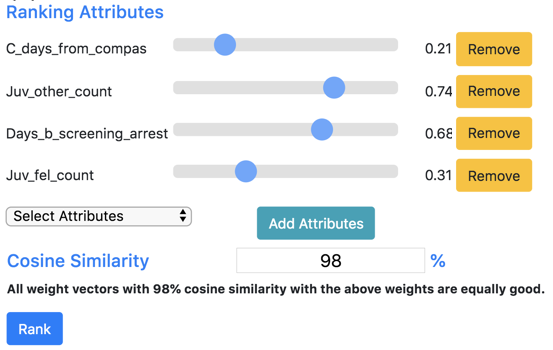
\includegraphics[width=\textwidth]{figs/m3.png}
    \vspace{-8mm}\caption{Specifying a weight vector}
    \label{fig:MR2}
\end{minipage}
\hfill
\begin{minipage}[t]{0.32\textwidth}
\centering
    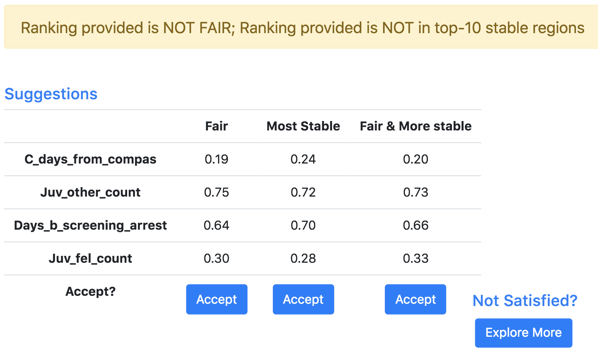
\includegraphics[width=\textwidth]{figs/m5.png}
    \vspace{-8mm}\caption{System results}
    \label{fig:MR3}
\end{minipage}
\end{figure*}



\vspace{-3mm}
\section{Coverage in Training Data}\label{sec:coverage} %2.5 to 3 pages
\vspace{-3mm}
So far in this paper, we discussed responsible design of scoring functions by a human expert.
Scoring models are also used for tasks such as classification and prediction
Such scoring models can be complex and are often determined using machine learning techniques. An essential piece to the learning is a labeled training dataset.
This dataset could be collected prospectively, such as through a survey or a scientific experiment. In such a case, a data scientist may be able to specify requirements such as representation and coverage.
However, more often than not, analyses are done with data that has been acquired independently, possibly through a process on which the data scientist has limited, or no, control. This is often called ``found data'' in the data science context.
It is generally understood that the training dataset must be representative of the distribution from which the actual test/production data will be drawn.  More recently, it has been recognized that it is not enough for the training data to be representative: it must include enough examples from less popular ``categories'', if these categories are to be handled well by the trained system.  Perhaps the best known story underlining the importance of this inclusion is the case of the ``google gorilla'' \cite{google-gorilla}.  An early image recognition algorithm released by Google had not been trained on enough dark-skinned faces.  When presented with an image of a dark African American, the algorithm labeled her as a ``gorilla''.  While Google very quickly patched the software as soon as the story broke, the question is what it could have done beforehand to avoid such a mistake in the first place.
The Google incident is not unique: there have been many other such incidents.
For example, Nikon introduced a camera feature to detect whether humans in the image have their eyes open -- to help avoid the all-too-common situation of the camera-subject blinking when the flash goes off resulting in an image with eyes closed.  Paradoxically for a Japanese company, their training data did not include enough East Asians, so that the software classified many (naturally narrow) open Asian eyes as closed~\cite{closed-eyes}.
% Similarly, HP webcams were not able to detect black faces~\cite{hp1} due to inadequate coverage in the training data~\cite{hp2}.

The problem becomes critical when the data is used for training models for data-driven algorithmic decision making.
For example, %judges, probation and parole officers are increasingly using algorithms to assess a criminal defendant's likelihood to re-offend~\cite{propublica}.
consider a tool designed to help judges in sentencing criminals by predicting how likely an individual is to re-offend. 
Such a tool can provide insightful signals for the judge and have the potential to make society safer.
On the other hand, a wrong signal can have devastating effects on individuals' lives.
So it is important to make sure that the tool is trained on data that includes adequate representation of individuals similar to each person that will be scored by it.
In \cite{asudeh2019assessing}, we study a real dataset of criminals used for building such a tool, published by Propublica~\cite{propublica}. We demonstrate that a model with an acceptable overall accuracy had an accuracy worse than random guess for Hispanic females, due to inadequate representation.

While Google's resolution to the gorilla incident was to ``ban gorillas''~\cite{google-gorilla-resolution}, a better solution is to ensure that the training data has enough entries in each category.
Referring to the issue as ``disparate predictive accuracy'', \cite{chen2018my} also highlights that the problem often is due to the insufficient or skewed sample sizes.
If the only category of interest were race, as in (most of) the examples above, there are only a handful of categories and this problem is easy.
However, in general, objects can have tens of attributes of interest, all of which could potentially be used to categorize the objects.  
For example, survey scientists use multiple demographic variables to characterize respondents, including race, sex, age, economic status, and geographic location.
Whatever be the mode of data collection for the analysis task at hand, we must ensure that there are enough entries in the dataset for each object category.  
Drawing inspiration from the literature on diversity \cite{diversity-jag}, we refer to this concept as {\em coverage}.

Lack of coverage in a dataset also opens up the room for adversarial attacks~\cite{biggio2013evasion}. The goal in an adversarial attack is to generate examples that are misclassified by a trained model.
Poorly covered regions in the training data provide the adversary with opportunities to create such examples.
For instance, consider the gorilla incident again. Knowing that black people are under-represented in the dataset gives the adversary the information that the models trained using this dataset are not well-trained for this category. The adversary can use this information to generate examples that are misclassified by the model.

Our objective here is two-fold.
First, we want to help the dataset users to  assess the coverage, as a characterization, of a given dataset, in order to understand such vulnerabilities.
For example, we use information about lack of coverage as a widget in the nutritional label~\cite{yang2018nutritional} of a dataset, in our MithraLabel system\footnote{http://mithra.eecs.umich.edu/demo/label/}\cite{sun2019mithralabel}.
Once the lack of coverage has been identified, next we would like to help data owners improve coverage by identifying the smallest number of additional data points needed to hit all the ``large uncovered spaces''.


Given multiple attributes, each with multiple possible values, we have a combinatorial number of possible {\em patterns}, as we call  combinations of values for some or all attributes.  Depending on the size and skew in the dataset, the coverage of the patterns will vary.  Given a dataset, our first problem is to efficiently identify patterns that do not have sufficient coverage (the learned model may perform poorly in portions of the attribute space corresponding to these patterns of attribute values).  It is straightforward to do this using space and time proportional to the total number of possible patterns.  Often, the number of patterns with insufficient coverage may be far fewer.  In~\cite{asudeh2019assessing}, we develop techniques, inspired from set enumeration and association rule mining ({\em apriori})~\cite{apriori}, to make this determination efficient.

A more interesting question for the dataset owners is what they can do about lack of coverage.
Given a list of patterns with insufficient coverage, they may try to fix these, for example by acquiring additional data.  In the ideal case, they will be able to acquire enough additional data to get sufficient coverage for all patterns.  However, acquiring data has costs, for data collection, integration, transformation, storage, etc.  Given the combinatorial number of patterns, it may just not be feasible to cover all of them in practice.  Therefore, we may seek to make sure that we have adequate coverage for at least any combination of $\ell$ attributes, where we call $\ell$ the {\em maximum covered level}.
Alternatively, we could identify important pattern combinations by means of a {\em value count}, indicating how many combinations of attribute values match that pattern.
Hence, our goal becomes to determine the patterns for the minimum number of items we must add to the dataset to reach a desired maximum covered level or to cover all patterns with at least a specified minimum value count.
%how a transformation to the frequent item-set problem can help in efficiently solving the problem.

We consider the low-dimensional categorical (sensitive) attributes $\mathcal{A} = \{A_1$, $A_2$, ..., $A_d\}$ such as {\tt \small race}, {\tt \small gender}, and {\tt \small age} for studying coverage. Where attributes are continuous valued or of high cardinality, we consider using techniques such as (a) bucketization: putting similar values into the same bucket, or (b) considering the hierarchy of attributes in the data cube for reducing the cardinality of any one attribute.
To capture lack of coverage in the dataset, we define a pattern $P$ as a vector of size $d$, in which $P[i]$ is either $X$ (meaning that its value is unspecified) or is a value of attribute $A_i$. We name the elements with value $X$ as non-deterministic and the others as deterministic.
We say an item $t$  {\em matches} a pattern $P$ (written as $M(t,P)= \top$), if for all $i$ for which $P[i]$ is deterministic, $t[i]$ is equal to $P[i]$.
For example, consider the pattern $P$ = $X1X0$ on four binary attributes $A_1$ to $A_4$.
It describes the value combinations that have the value 1 on $A_2$ and 0 on $A_4$.
Hence, for example, $t_1=[1,1,0,0]$ matches $P$, while $t_3=[1,0,1,0]$ does not match it, because $P[2]=1$ and $t_3[2]=0$.
Using the patterns to describe the space of value combinations, we define the coverage of a pattern $P$ as the number of items in $\mathcal{D}$ that match it.
We say a pattern $P$ is dominated by another pattern $P'$ if all value combinations matching it also match $P'$.
Our (lack of coverage) identification problem is to discover {\em Maximal Uncovered Patterns} (MUPs), the set of uncovered patterns (patterns with coverage less than a threshold) that are not dominated by another uncovered pattern.
This problem is \#P-complete.
At a high level, we define a directed acyclic graph (DAG) that captures the domination relation between the patterns and transform the problem into an enumeration on this graph while using the monotonicity property of coverage for pruning the search space.

We note that not all combinations of attribute values are of interest.  Some may be extremely unlikely, or even infeasible.  For example, we may find few people with attribute {\tt \small age} as ``teen'' and attribute {\tt \small education} as ``graduate degree''.
A human expert, with sufficient domain knowledge, is required to be in the loop for (i) identifying the attributes of interest, over which coverage is studied, (ii) setting up a {\em validation oracle} that identifies the value combinations that are not realistic, and (iii) identifying the uncovered patterns and the granularity of patterns that should get resolved during the coverage enhancement.

Our coverage enhancement problem is: given a dataset $\mathcal{D}$, its set of material MUPs $\mathcal{M}_\mathcal{D}$, and a positive integer number $\lambda$, to determine the minimum set of additional tuples to collect such that, after the data collection, the maximum number of deterministic values in any MUP is at least $\lambda$. The problem, using a polynomial-time reduction from the vertex cover problem, turns out to be NP-complete. 
Since a single tuple could contribute to the coverage of multiple patterns, we shall show that this problem translates to a hitting set~\cite{vazirani2013approximation} instance. Using this transformation, we show that the greedy approach provides a logarithmic approximation-ratio for the problem. Given the exponential number of value combinations, the direct implementation of hitting set techniques can be very expensive. Hence, we also provide an efficient implementation of the greedy approach.
\vspace{-3mm}\section{Final Remarks}\label{sec:conclusion2}
In this article we explained our results towards responsible data-driven decision making in score-based systems.
The scores, in these systems, are obtained by combining some features using either machine learning models or human-designed weight vectors.
We provided our results for (i) assisting the experts to design fair and stable rankings, and (ii) assessing and enhancing coverage in a (given) training dataset for tasks such as classification.

So far, in (i) our focus has been on ranking, where the scores are used for comparing the items in a pool. Human-designed scores are also used for tasks such as classification.
Extending our results for these tasks is part of our future work.
Also, we would like to adopt the proposed techniques for linear machine learning models.
The idea is to first train a machine learning model and then adjust the model to, for example, satisfy some fairness criteria. A similar idea can also be applied for designing ensemble methods for combining the outcome of multiple ML models.
In (ii), we used a fixed threshold across different value combinations, representing ``minor subgroups''.
We consider further investigations on identifying threshold value and minor subgroups for future work.
We will also investigate other properties (in addition to coverage) for assessing and enhancing the fitness of training data for responsible data science tasks.




% \bibliographystyle{unsrt}
% \small
% \bibliography{ref}

\begin{thebibliography}{10}
\itemsep=1pt
\begin{small}
\vspace{-3mm}

\bibitem{marcus2011human}
A.~Marcus, E.~Wu, D.~Karger, S.~Madden, and R.~Miller.
\newblock Human-powered sorts and joins.
\newblock {\em PVLDB}, 5(1):13--24, 2011.

\bibitem{asudeh2015pareto}
A.~Asudeh, G.~Zhang, N.~Hassan, C.~Li, and G.~V. Zaruba.
\newblock Crowdsourcing pareto-optimal object finding by pairwise comparisons.
\newblock In {\em CIKM}, pages 753--762. ACM, 2015.

\bibitem{fifa}
FIFA.
\newblock Fifa/coca-cola world ranking procedure.
\newblock www.fifa.com/fifa-world-ranking/procedure/men.html, 2008.

\bibitem{asudeh2019designing}
A.~Asudeh, H.~Jagadish, J.~Stoyanovich, and G.~Das.
\newblock Designing fair ranking schemes.
\newblock In {\em SIGMOD}. ACM, 2019.

\bibitem{salimi2019capuchin2}
B.~Salimi, L.~Rodriguez, B.~Howe, and D.~Suciu.
\newblock Capuchin: Causal database repair for algorithmic fairness.
\newblock In {\em SIGMOD}. ACM, 2019.

\bibitem{asudeh2016query}
A.~Asudeh, N.~Zhang, and G.~Das.
\newblock Query reranking as a service.
\newblock {\em PVLDB}, 9(11):888--899, 2016.

\bibitem{Gladwell11Order}
M.~Gladwell.
\newblock The order of things: What college rankings really tell us.
\newblock {\em The New Yorker Magazine}, 2011.

\bibitem{propublica}
J.~Angwin, J.~Larson, S.~Mattu, and L.~Kirchner.
\newblock Machine bias: Risk assessments in criminal sentencing.
\newblock {\em ProPublica}, 2016.

\bibitem{friedler2016possibility}
S.~A. Friedler, C.~Scheidegger, and S.~Venkatasubramanian.
\newblock On the (im) possibility of fairness.
\newblock {\em arXiv preprint arXiv:1609.07236}, 2016.

\bibitem{narayanan2018translation}
A.~Narayanan.
\newblock Translation tutorial: 21 fairness definitions and their politics.
\newblock In {\em FAT*}, 2018.

\bibitem{hardt2016equality2}
M.~Hardt, E.~Price, and N.~Srebro.
\newblock Equality of opportunity in supervised learning.
\newblock In {\em NIPS}, pages 3315--3323, 2016.

\bibitem{dwork2012fairness2}
C.~Dwork, M.~Hardt, T.~Pitassi, O.~Reingold, and R.~Zemel.
\newblock Fairness through awareness.
\newblock In {\em ITCS}, 2012.

\bibitem{edelsbrunner}
H.~Edelsbrunner.
\newblock {\em Algorithms in combinatorial geometry}, volume~10.
\newblock Springer Science \& Business Media, 2012.

\bibitem{redlining}
T.~Jan.
\newblock Redlining was banned 50 years ago. it’s still hurting minorities
  today.
\newblock Washington Post, 2018.

\bibitem{yang2018nutritional}
K.~Yang, J.~Stoyanovich, A.~Asudeh, B.~Howe, H.~Jagadish, and G.~Miklau.
\newblock A nutritional label for rankings.
\newblock In {\em SIGMOD}, pages 1773--1776. ACM, 2018.

\bibitem{asudeh2018obtaining}
A.~Asudeh, H.~Jagadish, G.~Miklau, and J.~Stoyanovich.
\newblock On obtaining stable rankings.
\newblock {\em PVLDB}, 12(3):237--250, 2018.

\bibitem{tang2017determining}
B.~Tang, K.~Mouratidis, and M.~L. Yiu.
\newblock Determining the impact regions of competing options in preference
  space.
\newblock In {\em SIGMOD}, 2017.

\bibitem{montecarlo}
C.~P. Robert.
\newblock {\em Monte carlo methods}.
\newblock Wiley Online Library, 2004.

\bibitem{rrr}
A.~Asudeh, A.~Nazi, N.~Zhang, G.~Das, and H.~Jagadish.
\newblock {RRR}: Rank-regret representative.
\newblock In {\em SIGMOD}. ACM, 2019.

\bibitem{muller1959note}
M.~E. Muller.
\newblock A note on a method for generating points uniformly on n-dimensional
  spheres.
\newblock {\em CACM}, 2(4), 1959.

\bibitem{marsaglia1972choosing}
G.~Marsaglia et~al.
\newblock Choosing a point from the surface of a sphere.
\newblock {\em The Annals of Math. Statistics}, 43(2), 1972.

\bibitem{lucidl1989random}
S.~Lucidl and M.~Piccioni.
\newblock Random tunneling by means of acceptance-rejection sampling for global
  optimization.
\newblock {\em Journal of optimization theory and applications},
  62(2):255--277, 1989.

\bibitem{guan2019mithraranking}
Y.~Guan, A.~Asudeh, P.~Mayuram, H.~Jagadish, J.~Stoyanovich, G.~Miklau, and
  G.~Das.
\newblock Mithraranking: A system for responsible ranking design.
\newblock In {\em SIGMOD}, 2019.

\bibitem{google-gorilla}
M.~Mulshine.
\newblock A major flaw in google's algorithm allegedly tagged two black
  people's faces with the word 'gorillas'.
\newblock Business Insider, 2015.

\bibitem{closed-eyes}
A.~Rose.
\newblock Are face-detection cameras racist?
\newblock Time Business, 2010.

\bibitem{asudeh2019assessing}
A.~Asudeh, Z.~Jin, and H.~Jagadish.
\newblock Assessing and remedying coverage for a given dataset.
\newblock {\em ICDE}, 2019.

\bibitem{google-gorilla-resolution}
A.~Hern.
\newblock Google's solution to accidental algorithmic racism: ban gorillas.
\newblock The Guardian, 2018.

\bibitem{chen2018my}
I.~Chen, F.~D. Johansson, and D.~Sontag.
\newblock Why is my classifier discriminatory?
\newblock In {\em NeurIPS}, 2018.

\bibitem{diversity-jag}
M.~Drosou, H.~Jagadish, E.~Pitoura, and J.~Stoyanovich.
\newblock Diversity in big data: A review.
\newblock {\em Big data}, 5(2), 2017.

\bibitem{biggio2013evasion}
B.~Biggio, I.~Corona, D.~Maiorca, B.~Nelson, N.~{\v{S}}rndi{\'c}, P.~Laskov,
  G.~Giacinto, and F.~Roli.
\newblock Evasion attacks against machine learning at test time.
\newblock In {\em ECML PKDD}, 2013.

\bibitem{sun2019mithralabel}
C.~Sun, A.~Asudeh, H.~V. Jagadish, B.~Howe, and J.~Stoyanovich.
\newblock Mithralabel: Flexible dataset nutritional labels for responsible data
  science.
\newblock In {\em CIKM}. ACM, 2019.

\bibitem{apriori}
R.~Agrawal and R.~Srikant.
\newblock Fast algorithms for mining association rules.
\newblock In {\em VLDB}, 1994.

\bibitem{vazirani2013approximation}
V.~V. Vazirani.
\newblock {\em Approximation algorithms}.
\newblock Springer Science \& Business Media, 2013.

\end{small}
\end{thebibliography}
\end{document}
